\documentclass[11pt, a4paper]{article}
\usepackage{pdfpages}
\usepackage{parallel}
\usepackage[T2A]{fontenc}
\usepackage{ucs}
\usepackage[utf8x]{inputenc}
\usepackage[polish,english,russian]{babel}
\usepackage{hyperref}
\usepackage{rotating}
\usepackage[inner=2cm,top=1.8cm,outer=2cm,bottom=2.3cm,nohead]{geometry}
\usepackage{listings}
\usepackage{graphicx}
\usepackage{wrapfig}
\usepackage{longtable}
\usepackage{indentfirst}
\usepackage{array}
\usepackage{tikzsymbols}
\usepackage{soul}
\usepackage[ruled,vlined]{algorithm2e}
%\counterwithout{figure}{section} 

\usepackage{url}
\makeatletter
\g@addto@macro{\UrlBreaks}{\UrlOrds}
\makeatother

\newcolumntype{P}[1]{>{\raggedright\arraybackslash}p{#1}}
\frenchspacing
\usepackage{fixltx2e} %text sub- and superscripts
\usepackage{icomma} % коскі ў матэматычным рэжыме
\PreloadUnicodePage{4}

\newcommand{\longpage}{\enlargethispage{\baselineskip}}
\newcommand{\shortpage}{\enlargethispage{-\baselineskip}}

\def\switchlang#1{\expandafter\csname switchlang#1\endcsname}
\def\switchlangbe{
\let\saverefname=\refname%
\def\refname{Літаратура}%
\def\figurename{Іл.}%
}
\def\switchlangen{
\let\saverefname=\refname%
\def\refname{References}%
\def\figurename{Fig.}%
}
\def\switchlangru{
\let\saverefname=\refname%
\let\savefigurename=\figurename%
\def\refname{Литература}%
\def\figurename{Рис.}%
}

\hyphenation{admi-ni-stra-tive}
\hyphenation{ex-pe-ri-ence}
\hyphenation{fle-xi-bi-li-ty}
\hyphenation{Py-thon}
\hyphenation{ma-the-ma-ti-cal}
\hyphenation{re-ported}
\hyphenation{imp-le-menta-tions}
\hyphenation{pro-vides}
\hyphenation{en-gi-neering}
\hyphenation{com-pa-ti-bi-li-ty}
\hyphenation{im-pos-sible}
\hyphenation{desk-top}
\hyphenation{elec-tro-nic}
\hyphenation{com-pa-ny}
\hyphenation{de-ve-lop-ment}
\hyphenation{de-ve-loping}
\hyphenation{de-ve-lop}
\hyphenation{da-ta-ba-se}
\hyphenation{plat-forms}
\hyphenation{or-ga-ni-za-tion}
\hyphenation{pro-gramming}
\hyphenation{in-stru-ments}
\hyphenation{Li-nux}
\hyphenation{sour-ce}
\hyphenation{en-vi-ron-ment}
\hyphenation{Te-le-pathy}
\hyphenation{Li-nux-ov-ka}
\hyphenation{Open-BSD}
\hyphenation{Free-BSD}
\hyphenation{men-ti-on-ed}
\hyphenation{app-li-ca-tion}

\def\progref!#1!{\texttt{#1}}
\renewcommand{\arraystretch}{2} %Іначай формулы ў матрыцы зліпаюцца з лініямі
\usepackage{array}

\def\interview #1 (#2), #3, #4, #5\par{

\section[#1, #3, #4]{#1 -- #3, #4}
\def\qname{LVEE}
\def\aname{#1}
\def\q ##1\par{{\noindent \bf \qname: ##1 }\par}
\def\a{{\noindent \bf \aname: } \def\qname{L}\def\aname{#2}}
}

\def\interview* #1 (#2), #3, #4, #5\par{

\section*{#1\\{\small\rm #3, #4. #5}}
\ifx\ParallelWhichBox\undefined%
    \addcontentsline{toc}{section}{#1, #3, #4}%
\else%
\ifnum\ParallelWhichBox=0%
    \addcontentsline{toc}{section}{#1, #3, #4}%
\fi\fi%

\def\qname{LVEE}
\def\aname{#1}
\def\q ##1\par{{\noindent \bf \qname: ##1 }\par}
\def\a{{\noindent \bf \aname: } \def\qname{L}\def\aname{#2}}
}

\newcommand{\interviewfooter}[1]{
\vskip 1em
\noindent \textit{#1}
}

\switchlang{ru}
\begin{document}

\title{1999 "--- Contour UniMouse}
\date{}
\maketitle
\selectlanguage{russian}
Мышь UniMouse была выпущена компанией Contour Design, специализирующейся исключительно на эргономических манипуляторах, для компьютеров Apple iMac, как замена для комплектной Apple USB mouse, из-за круглой формы известной как <<шайба>> (англ. <<puck>>). Многие критиковали Apple USB mouse за плохую эргономику, и через год после ее выхода на рынок последовал выпуск альтернативы от одного из лидеров в производстве эргономичных средств управления курсором \cite{pressrelease}.

\begin{figure}[h]
    \centering
    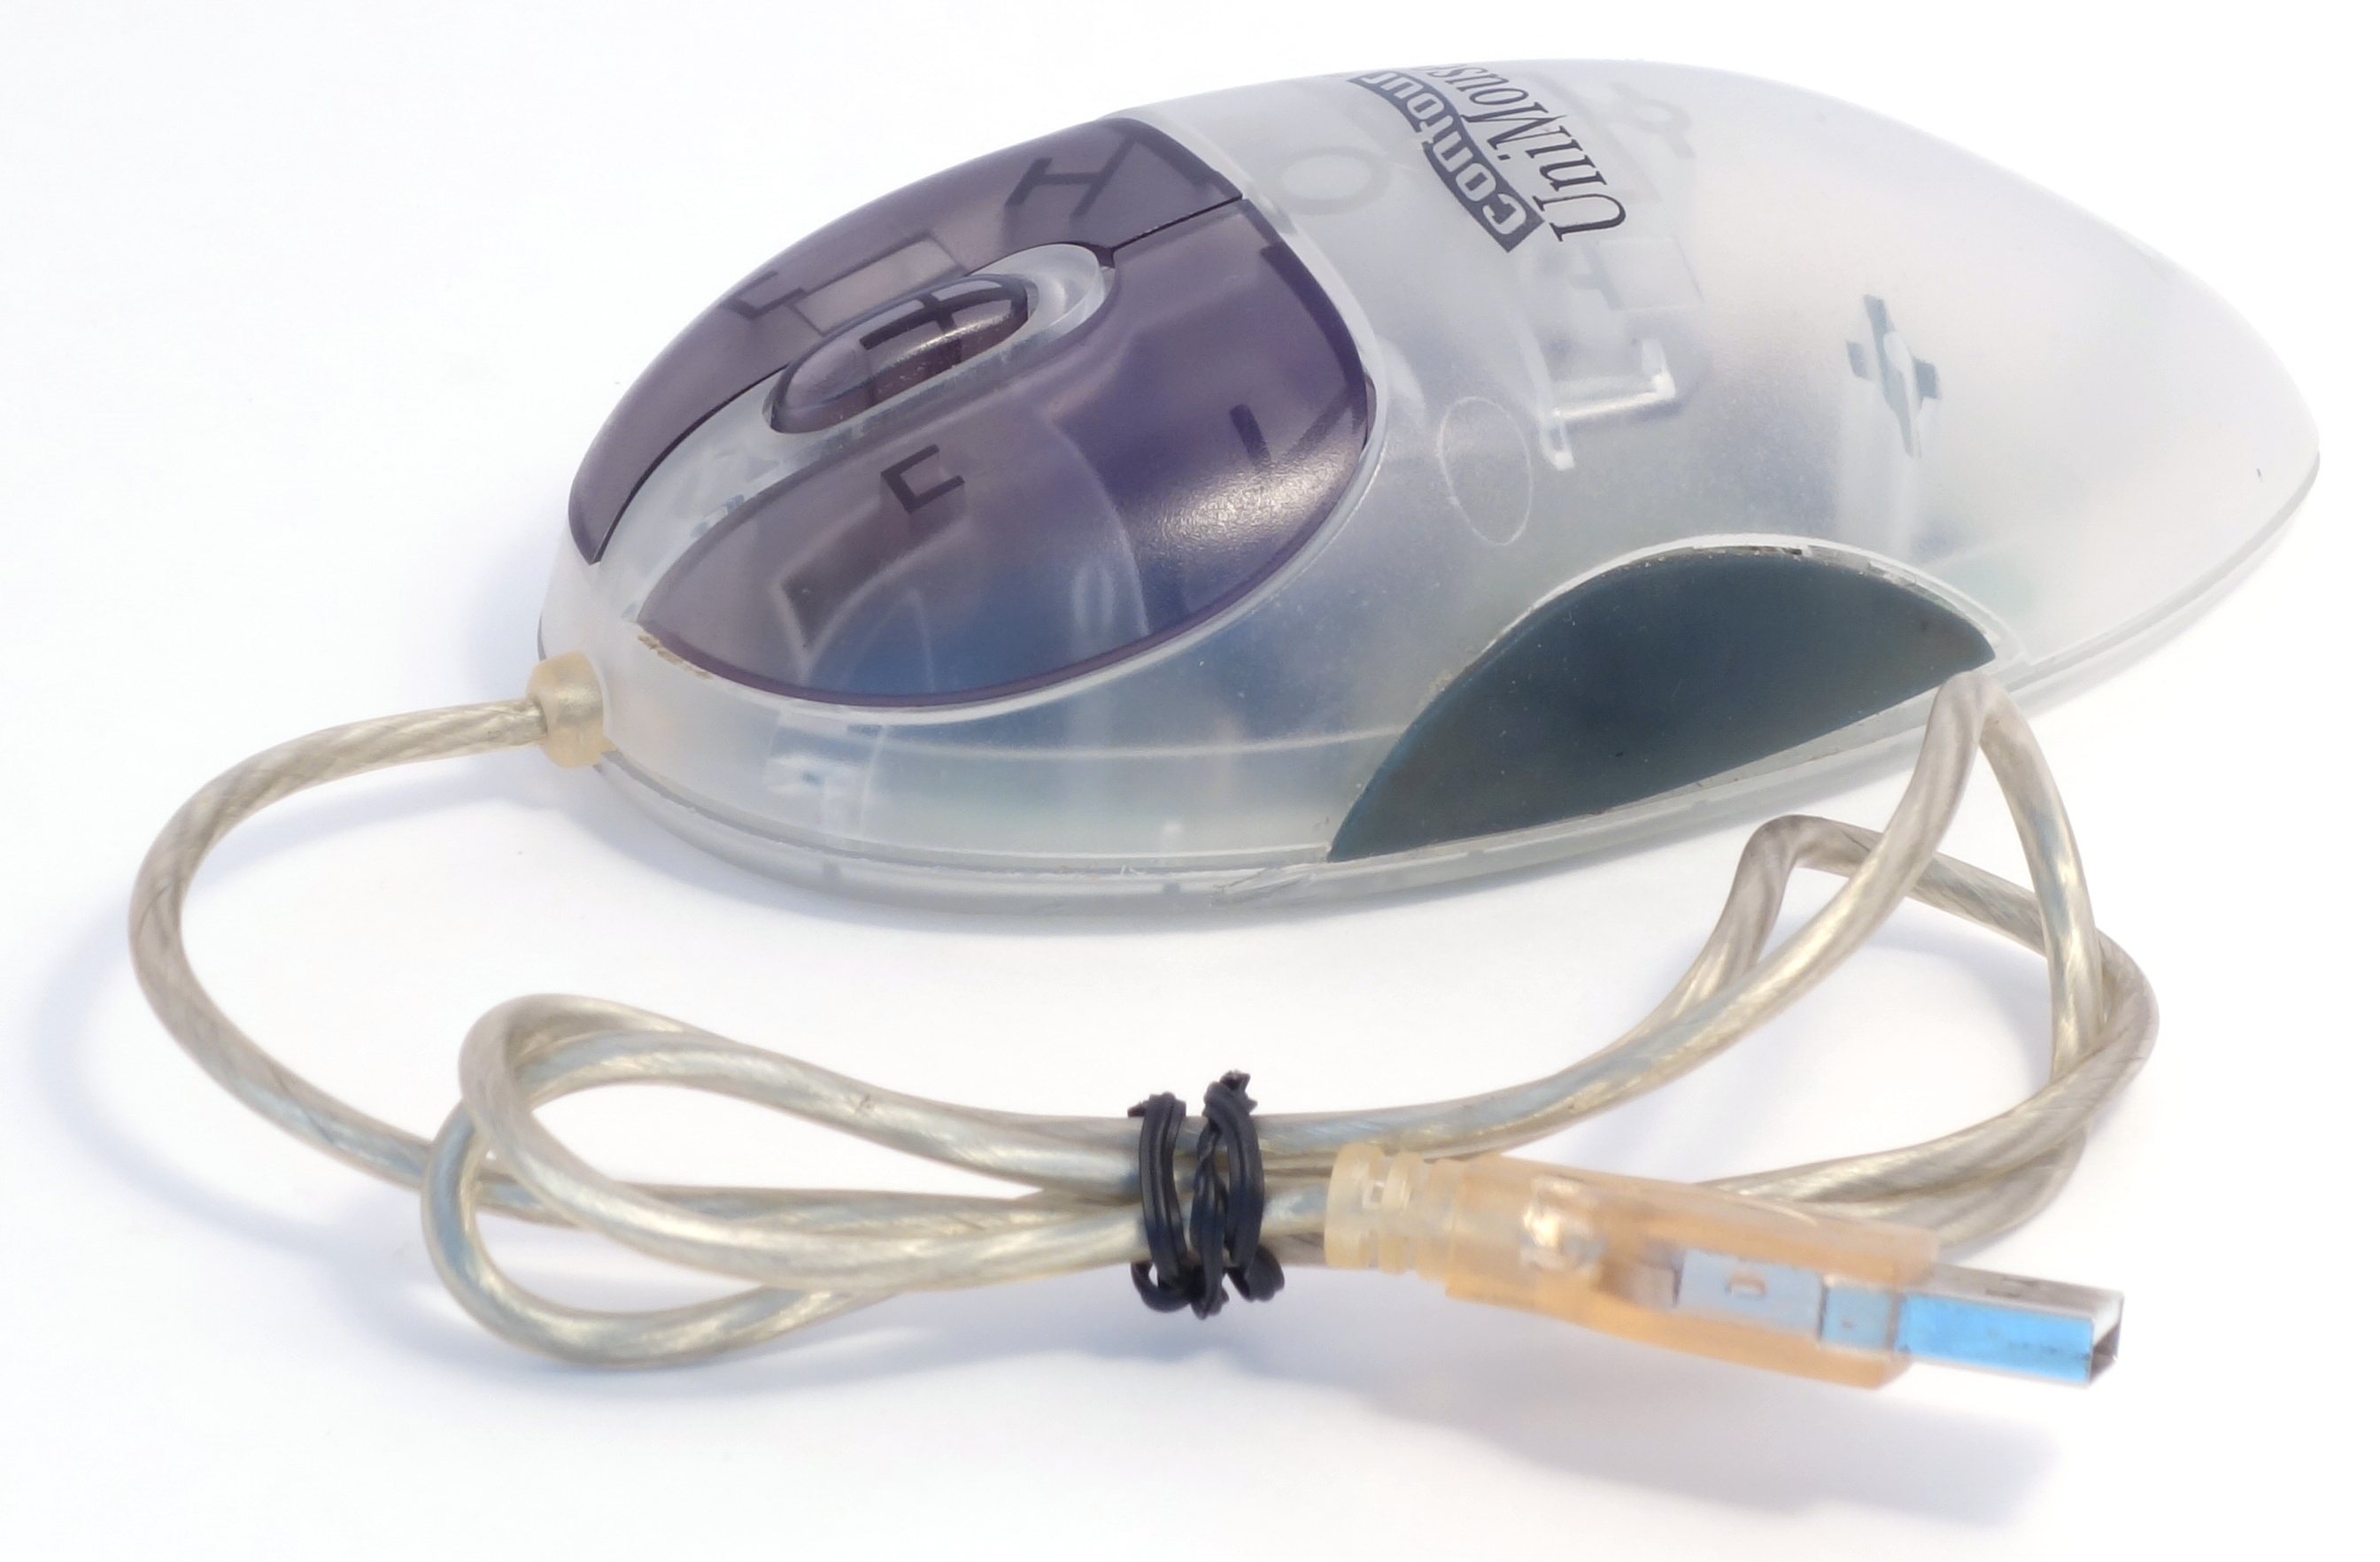
\includegraphics[scale=0.5]{1999_contour_unimouse/pic_30.jpg}
    \caption{Contour UniMouse}
    \label{fig:ContourUniMousePic}
\end{figure}

Мышь имеет полупрозрачный корпус, через который просвечивает печатная плата \ref{fig:ContourUniMouseTopAndBottom}, украшенный тонированными кнопками и принтом с названием мыши. Две крупные кнопки расположены в передней части корпуса. Между ними присутствует выпуклая третья кнопка, визуально стилизованная под колесо прокрутки. Нижняя часть мыши из прозрачного пластика выглядит вполне традиционно, включая ножки из низкофрикционного материала и съемное кольцо-защелку, позволяющее извлечь шар для чистки. По бокам корпуса размещены резиновые накладки для более комфортного захвата.

\begin{figure}[h]
    \centering
    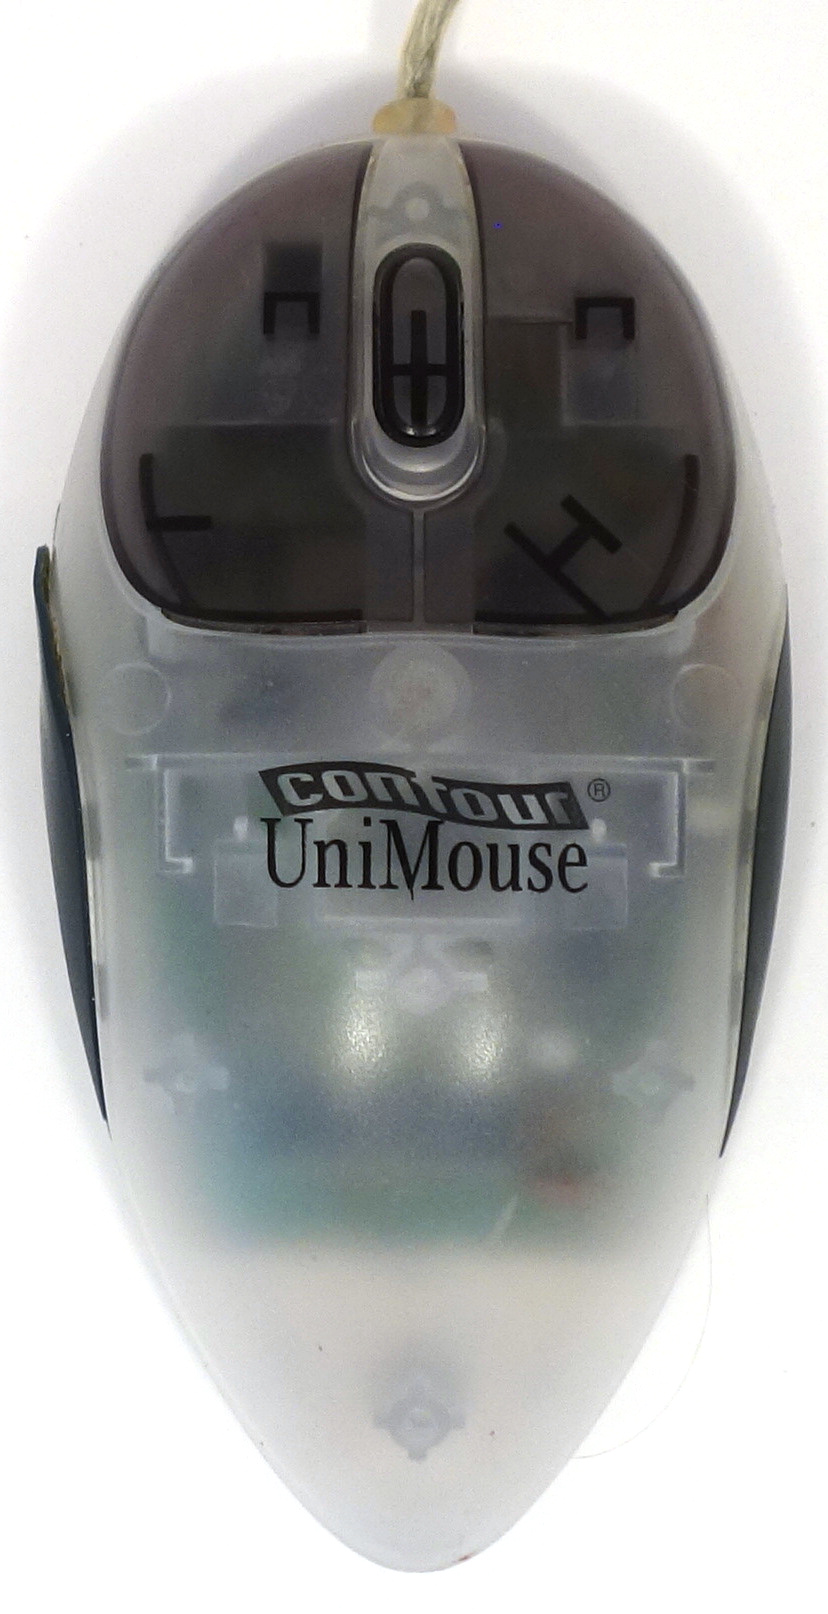
\includegraphics[scale=0.45]{1999_contour_unimouse/top_30.jpg}
    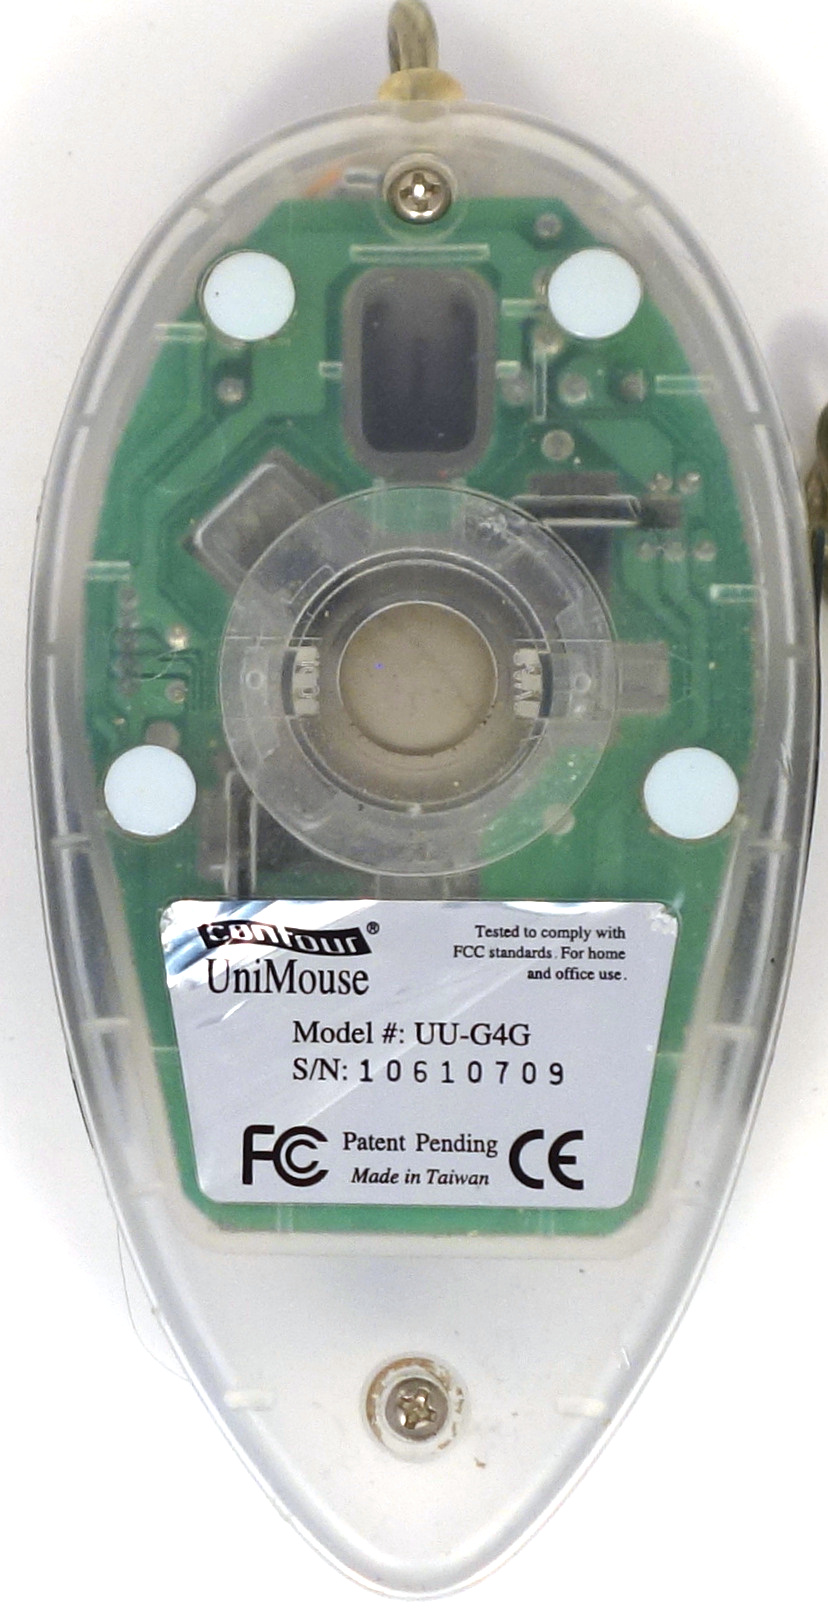
\includegraphics[scale=0.45]{1999_contour_unimouse/bottom_30.jpg}
    \caption{Contour UniMouse, вид сверху и снизу}
    \label{fig:ContourUniMouseTopAndBottom}
\end{figure}

Мышь имела несколько вариантов цветового оформления кнопок, резиновых накладок и надписи для соответствия вариантам оформления корпуса iMac \cite{web}.

Размеры мыши (в отличие от Apple USB mouse) средние, типичные для мышей конца девяностых (рис. \ref{fig:ContourUniMouseSize}).

\begin{figure}[h]
    \centering
    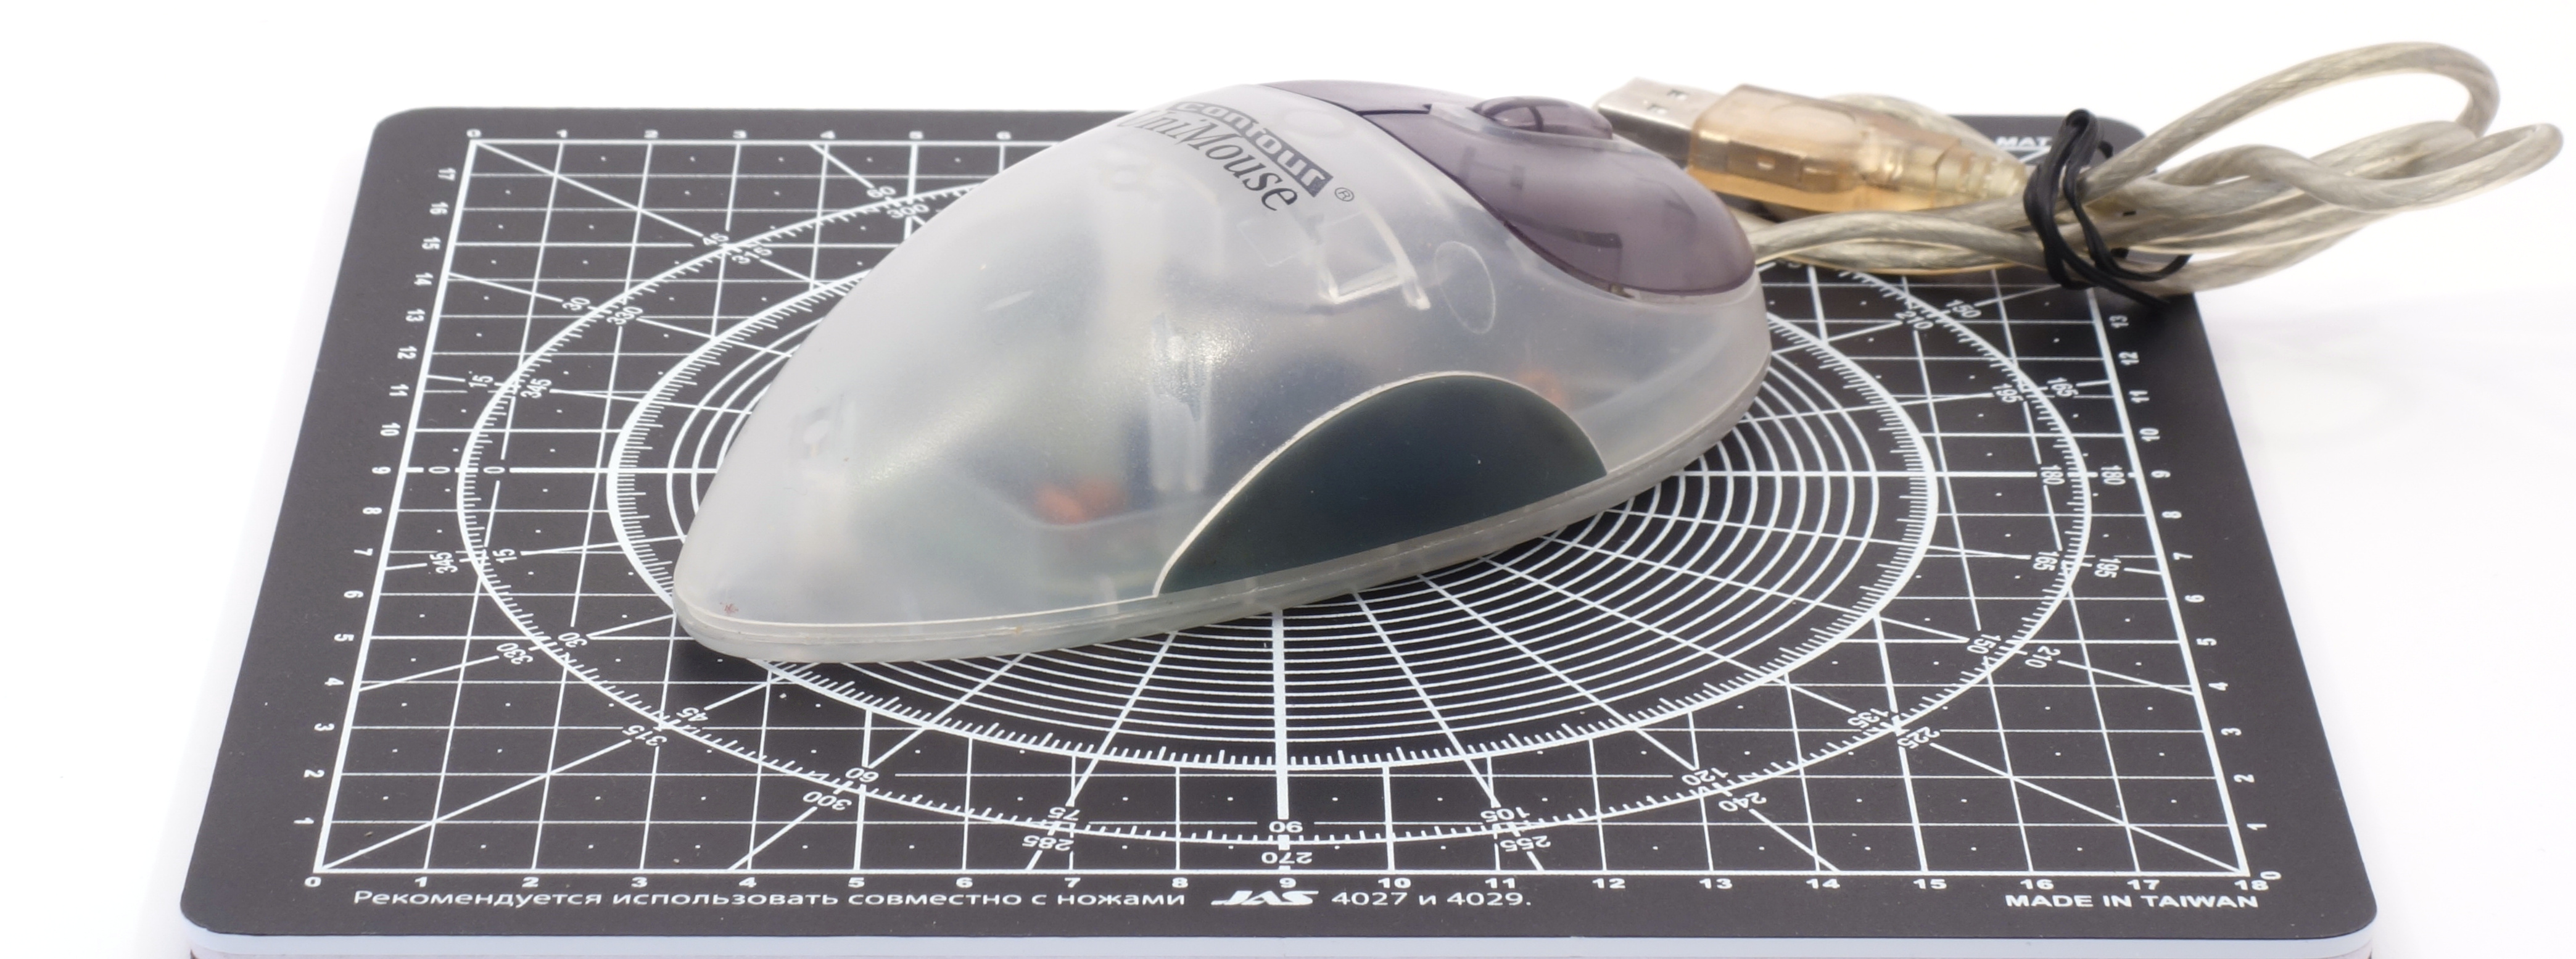
\includegraphics[scale=0.5]{1999_contour_unimouse/size_30.jpg}
    \caption{Contour UniMouse на размерном коврике с шагом сетки 1~см}
    \label{fig:ContourUniMouseSize}
\end{figure}

Благодаря симметричности мышь одинаково подходит как для левшей, так и для правшей. Учитывая специализацию Contour Design, не приходится удивляться тому, что рука комфортно лежит на мыши (рис. \ref{fig:ContourUniMouseHand}).

\begin{figure}[h]
    \centering
    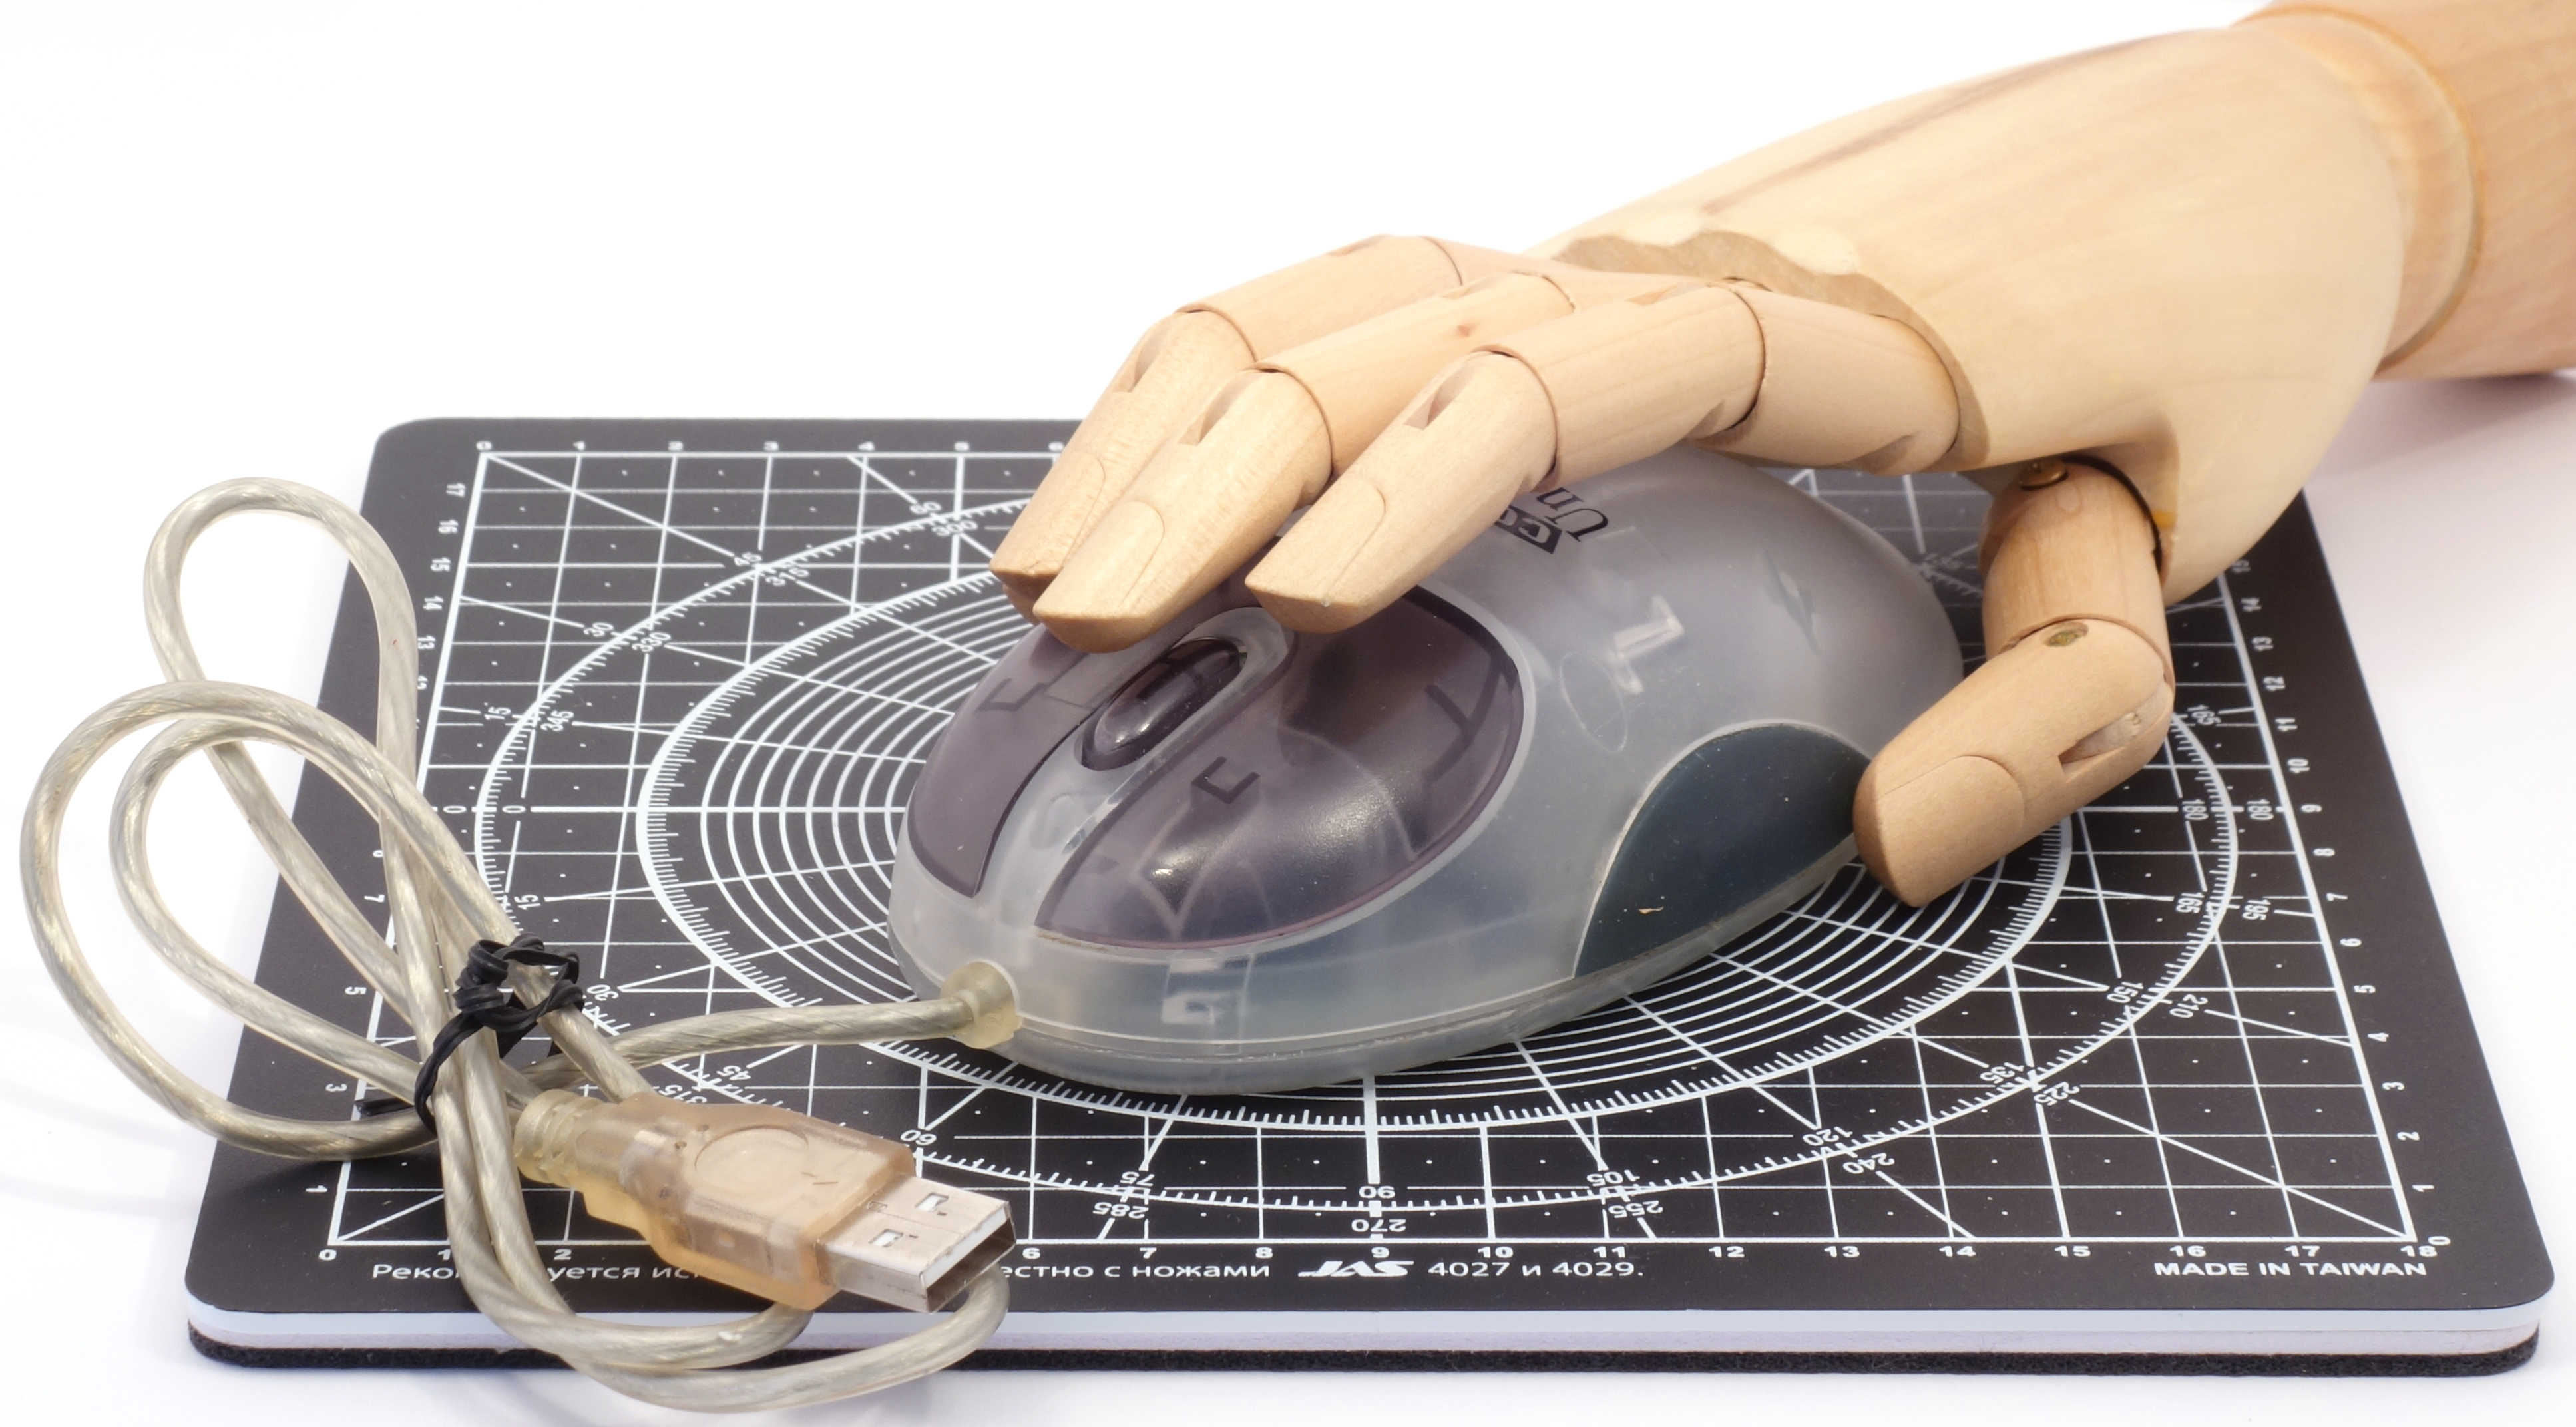
\includegraphics[scale=0.55]{1999_contour_unimouse/hand_30.jpg}
    \caption{Contour UniMouse с моделью руки человека}
    \label{fig:ContourUniMouseHand}
\end{figure}

В качестве незначительного недостатка \cite{mactoday} упоминает малую площадь опоры под запястье. Отсутствие колеса прокрутки компенсировалось программной реализацией: скроллинг в четырех направлениях осуществлялся перемещением мыши при нажатии на среднюю кнопку. Очевидно, что это решение трудно назвать идеальным: оно более трудоемко для пользователя, чем традиционный скроллинг, сама кнопка менее удобна, а кроме того требуется скачивать специально сконфигурированный драйвер и/или вспомогательное программное обеспечение с сайта производителя мыши. Однако в целом, для платформы Apple данная мышь была весьма качественным решением, компенсировавшим проблемную эргономику Apple USB mouse, для которой сторонними производителями выпускались даже специальные адаптеры-накладки, придававшие ей более продолговатую форму.

\begin{figure}[h]
    \centering
    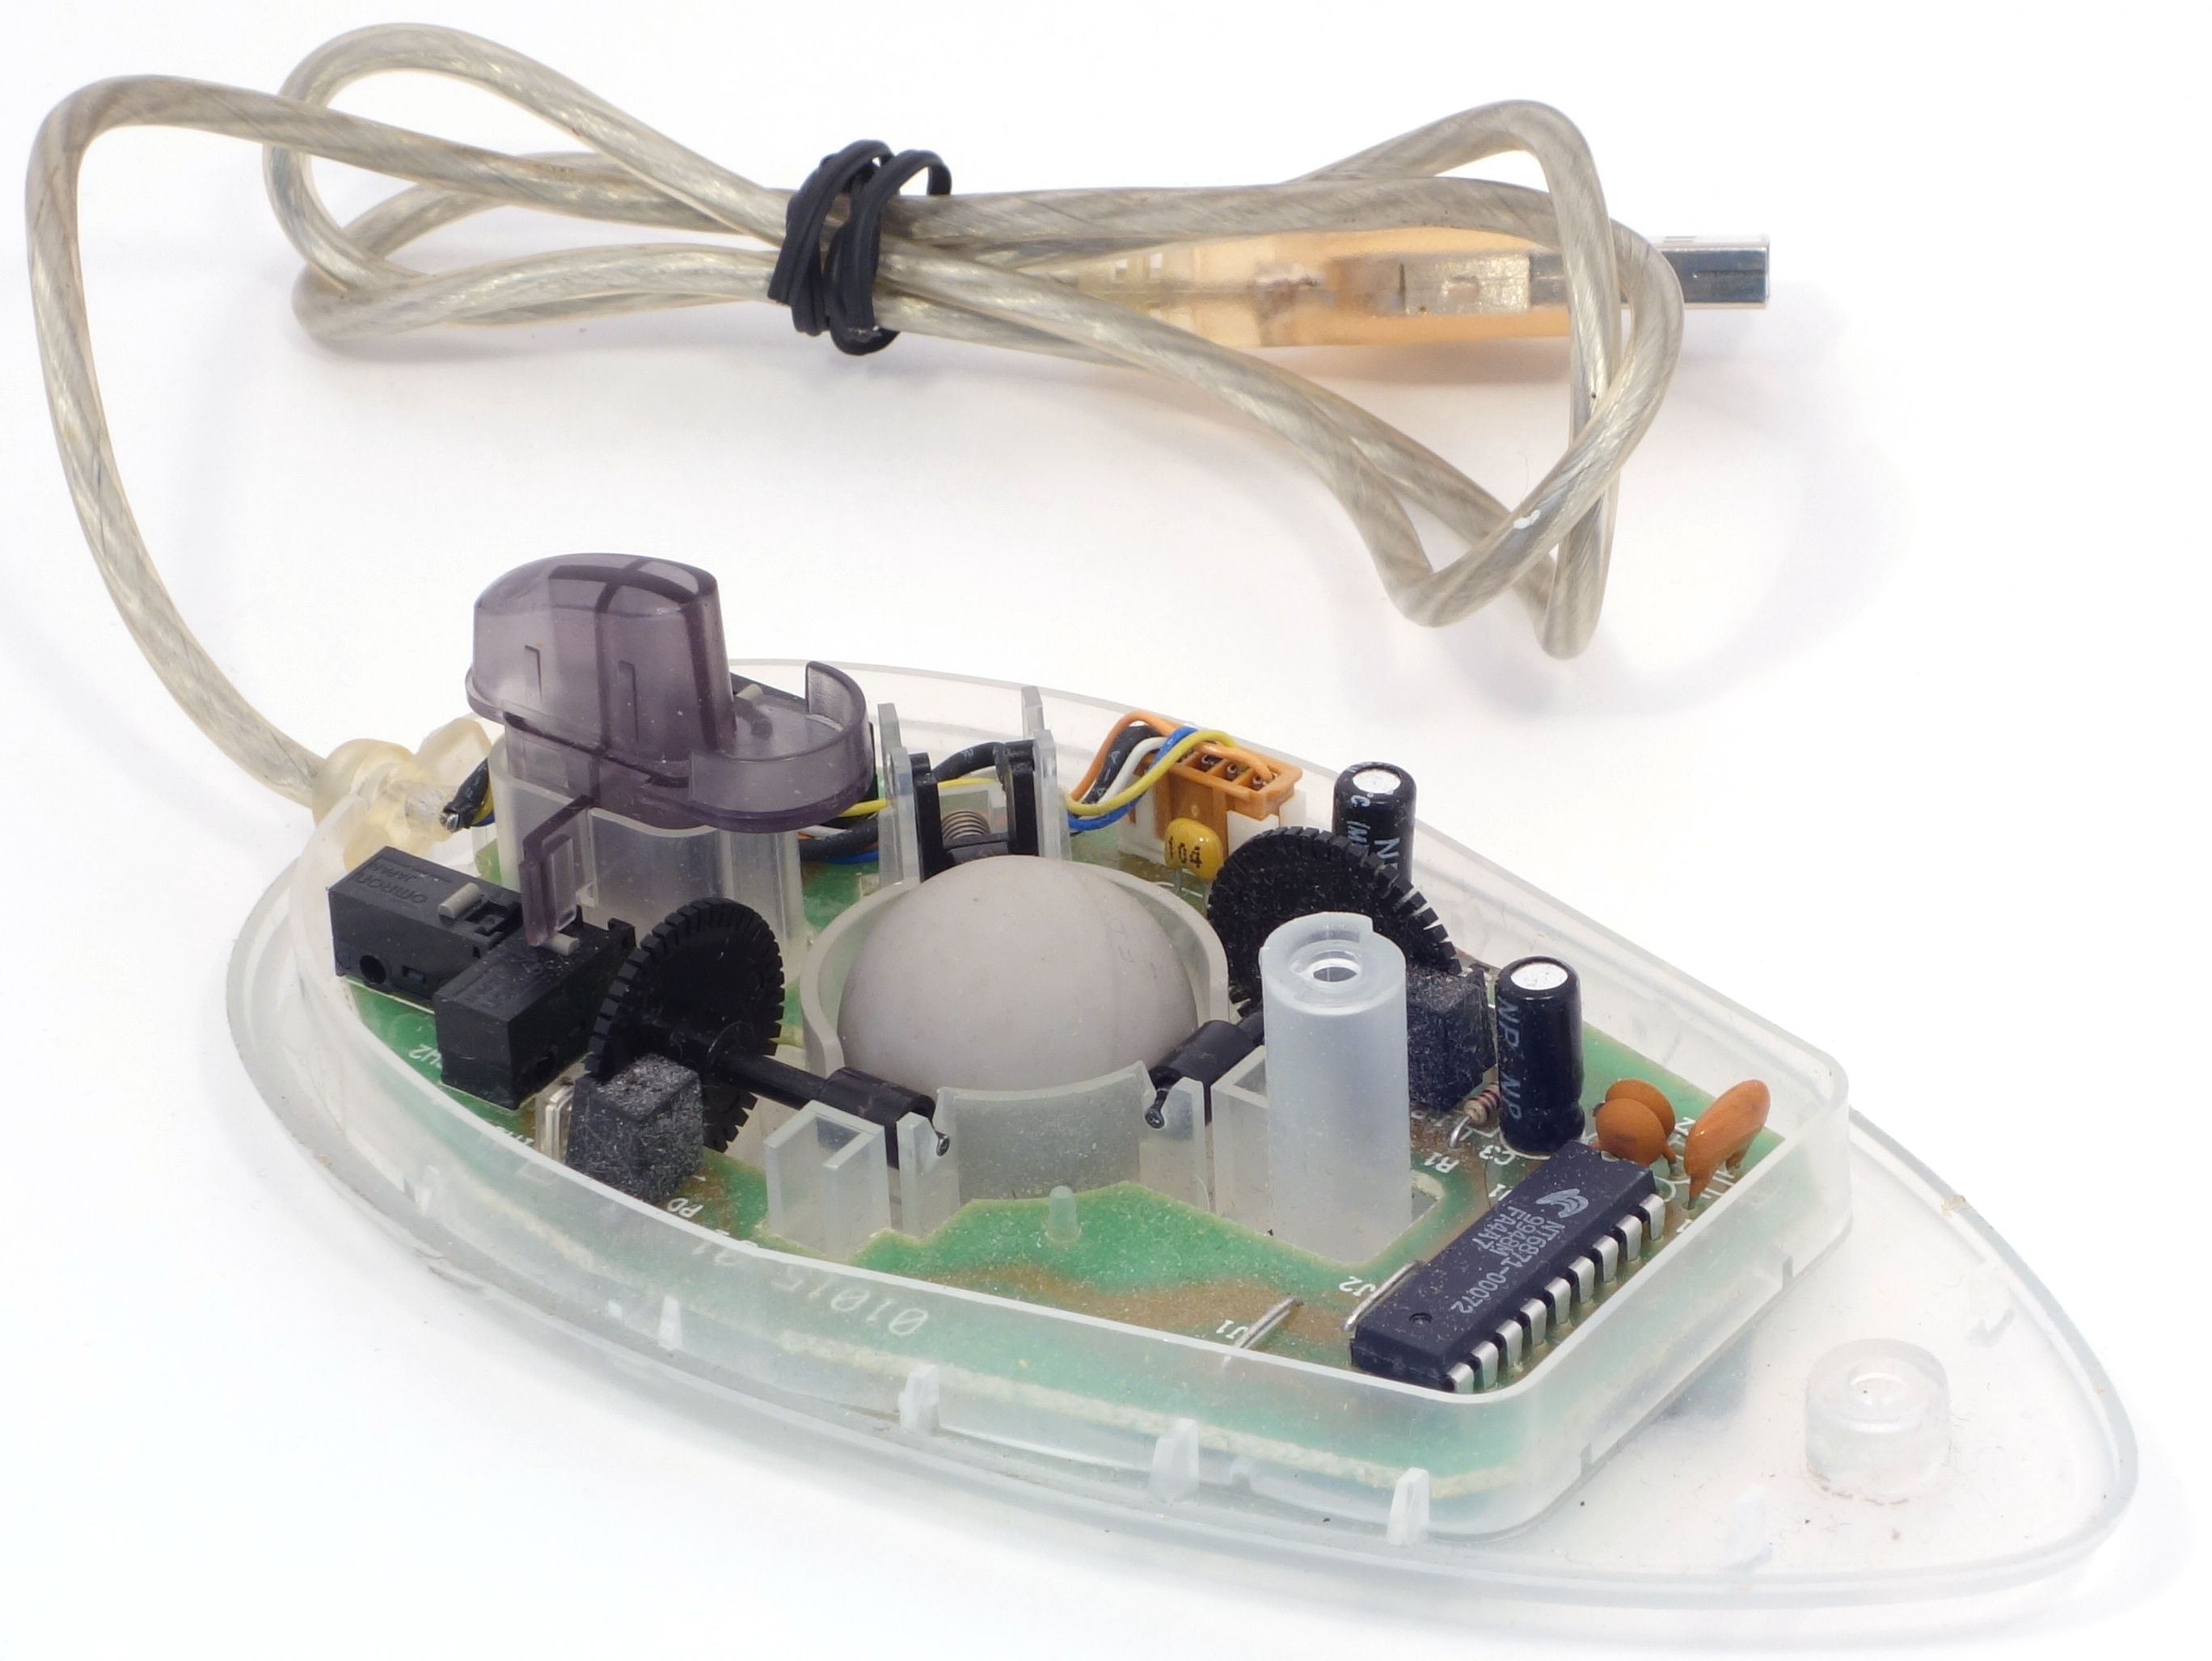
\includegraphics[scale=0.7]{1999_contour_unimouse/inside_30.jpg}
    \caption{Contour UniMouse, в разобранном виде}
    \label{fig:ContourUniMouseInside}
\end{figure}

Внутреннее устройство данной мыши показано на рис. \ref{fig:ContourUniMouseInside}, что позволяет классифицировать его как традиционную оптомеханическую конструкцию. Форма диска оптического прерывателя с зубцами вместо прорезей типична скорее для мышей более раннего периода, однако в данной модели частота зубцов заметно увеличена для большей разрешающей способности и соответствует частоте прорезей в прерывателях других достаточно качественных мышей конца девяностых. Вместе с тем в конструкции максимально используется пластик, отсутствуют дорогие механические элементы, что позволило вписать мышь в бюджетный ценовой диапазон (в пределах \$40).

\begin{thebibliography}{9}
    \bibitem{pressrelease} Contour UniMouse Press Releases "--- \url{http://www.contourdesign.com/unimouse_press.htm} 
    \bibitem{web} Contour UniMouse Home Page "--- \url{http://contourdesign.com/unimouse.htm}
    \bibitem{mactoday} Hemmel J. Contour UniMouse. Avoiding Apple's mouse trap // mac today, May/June 1999 \url{https://web.archive.org/web/20000619173033/http://mactoday.com/mayjun99/unimouse.html}
\end{thebibliography}

\end{document}
